Este capítulo contiene definiciones y resultados que ya han sido abordados en el curso Cadenas de Markov. No obstante, nos interesaremos también en simular cadenas de Markov de manera eficiente. También se propondrán algoritmos para simular la distribución invariante de una cadena.

\newp Para revisar el tema con mayor profundidad, se puede consultar  ``Markov Chains'' de J. Norris \cite{norris} o ``Processus de Markov et applications'' de E. Pardoux \cite{pardoux}.
\subsection{Recuerdo}
En esta sección recordaremos las bases de Cadenas de Markov. 
\subsubsection{Definición}
\begin{definition}[Cadena de Markov]
Sea $E$ un conjunto numerable, $P=(P_{xy})_{x,y\in E}$ matriz estocástica y $\lambda=(\lambda_x)_{x\in E}$ vector de probabilidad inicial.

La $(X_n)_{n\in N}$ sucesión de variables aleatorias con $X_n:\edp \to E$ se dice \textbf{Cadena de Markov} C.M.($\lambda,P$) (homog\'enea) si:
\begin{itemize}
    \item $\forall n \in N, \forall x_0,\dots,x_{n+1}\in E \, ,$
    $$ \P(X_{n+1}=x_{n+1}|X_n=x_n,\dots,X_0=x_0) = P_{x_n,x_n+1} \, .$$
    \item $\forall x_0\in E$, $\P(X_0=x_0)=\lambda_0 \, .$
\end{itemize}
\end{definition}

\begin{property}
Algunas consecuencias:
\begin{itemize}
    % \item $\P(X_{n+1}=x_{n+1}|X_n=x_n) = P_{x_nx_{n+1}}$ \, .
    \item $\P(X_{n+1}=y|X_n=x) = P_{xy}$ \, .
    \item $X$ es $CM(\lambda,P)$ si y solo si $$\P(X_0=x_0,\dots,X_n=x_n)=\lambda_{x_0}P_{x_0,x_1}\dots P_{x_{n-1}x_n}\, .$$
\end{itemize}
\end{property}

\subsubsection{Definiciones y propiedades importantes}
\begin{notation}
Denotaremos
\begin{itemize}
    \item $\P_\mu(\cdot)$ a la ley de $\xcm$ cuando $X_0\sim\lambda=\mu$ \, .
    \item $\P_x(\cdot)=\P_{\delta_x}(\cdot)$, con $\delta_x$ masa de Dirac en $x\in E$ \, .
\end{itemize}
\end{notation}

\begin{definition}[$x$ ``pasa'' a $y$]
Sea $X=\xcm$, decimos que $x$ ``pasa'' a $y$ si
$$\P_x(\exists n\geq 0 \tq X_n=y)>0 \, ,$$
y se denota $x\longrightarrow y$.
\end{definition}
\begin{remark}
$x\longleftrightarrow y$ es relación de equivalencia (donde $x\longleftrightarrow y$ si $x\longrightarrow y$ y $y\longrightarrow x$).
\end{remark}
\begin{definition}[Cadena irreducible]
Una cadena $X=\cm$ se dice irreducible si $E$ es la única clase de equivalencia para $\longleftrightarrow$ \, .
\end{definition}
\begin{property}[de Semigrupo]
Sea $X\sim\cm$, entonces $$ \P_X(X_n=y)=(P^n)_{xy} \, .$$
\end{property}
\begin{definition}[Filtración]
Sea $\edp$ un espacio de probabilidad. Sea $(\mathcal{F}_i)_{i\in\N}$ una familia de sub-$\sigma$-álgebras de $\mathcal{F}$. \\ Si $\forall i,j\in\N, i<j$ tenemos $$\mathcal{F}_i\subseteq\mathcal{F}_j \, ,$$
entonces $(\mathcal{F}_i)_{i\in\N}$ se dice una filtración.
\end{definition}
\begin{remark}
Sea $(X_n)_{n\in\N}$ C.M. familia $(\mathcal{F}_i)_{i\in\N}$, dada por $\mathcal{F}_n=\sigma(X_0,\dots,X_n)\, \forall n\in\N$, es una filtración.
\end{remark}
\begin{theorem}[Propiedad de Markov]
Sea $X\sim\cm$ entonces $\forall F:E^\N \to \R$ medible y acotada se tiene
% $$ \E(F(X_{n+1},X_{n+2},\dots)|X_0,\dots,X_n)=\E_{X_n}(F(X_1,X_2,\dots)) \, .$$
$$ \E(F(X_{n+1},X_{n+2},\dots)|\mathcal{F}_0,\dots,\mathcal{F}_n)=\E_{X_n}(F(X_1,X_2,\dots)) \espacio c.s.\, ,$$
donde $\mathcal{F}_n=\sigma(X_0,\dots,X_n)$\,.
\end{theorem}
% \begin{remark}
% La familia $\mathcal{F}_n=\sigma(X_0,\dots,X_n)$ es una filtración (i.e., $\mathcal{F}_n\subset\mathcal{F}_{n+1}\subset\dots\subset\mathcal{F}$)
% \end{remark}
\begin{definition}[Tiempo de parada]
Sea $(\mathcal{F}_i)_{i\in\N}$ una filtración y sea $\tau:\Omega\mapsto\N\cup\{\infty\}$ v.a.. $\tau$ se dice tiempo de parada si
$$\forall m\in\N,\espacio \{\tau\leq m\}\in\mathcal{F}_m \, .$$
\newline A la $\sigma$-álgebra $\mathcal{F}_\tau:=\{A\in\mathcal{F}:A\cap\{\tau\leq m\}\forall m \in \N\}$ se le dice su tribu asociada.
\end{definition}
\begin{theorem}[Propiedad de Markov Fuerte]
Sea $X\sim\cm$, entonces
$$ \E(F(X_{\tau+1},X_{\tau+2},\dots)|\mathcal{F}_\tau)=\E_{X_\tau}(F(X_1,\dots)) \mbox{ c.s. en }\{\tau<\infty\} \, .$$
\end{theorem}
\begin{remark}
El tiempo de retorno a $x\in E$ está dado por $\tau_X=\inf\{n\geq1:X_n=x\}$, y es un tiempo de parada.
\end{remark}
\begin{definition}[Recurrencia y Transiencia]
$x\in E$ se dice recurrente si:
$$ \P_x(\tau_x<\infty)=1 \, .$$
En caso contrario se dice transiente.
\end{definition}
\begin{remark}
Recurrencia es una propiedad de clase.
\end{remark}
\vspace{1cm}\\
\begin{proposition}
\beforeitemize
\begin{itemize}
    \item Una $CM(\lambda,P)$ irreducible se dice recurrente/transiente si $x\in E$ lo es.
    \item Toda $\cm$ irreducible en $E$ finito es recurrente.
\end{itemize}
\end{proposition}
\begin{theorem}
\label{theorem:visitas}
Sea $X\sim\cm$ y denotemos
$$ N_x:=\displaystyle\sum_{n\in\N}\mathbf{1}_{\{X_n=x\}} \, ,$$
que corresponde al \textbf{número de visitas} de la cadena al estado $x\in E$.
\newline Entonces son equivalentes:
\begin{itemize}
    \item $x\in E$ recurrente.
    \item $N_x=\infty \mbox{ }\P_X-{ c.s.}$.
    \item $\displaystyle\sum_{n\in \N}(P^n)_{xx}=\E_x(N_x)=\infty$.
\end{itemize}
\end{theorem}
\begin{definition}[Medida y Probabilidad Invariante]
Sea $X\sim\cm$, $\gamma=(\gamma_x)_{x\in E}$ con $\gamma_x\geq0$ se dice \textbf{medida invariante} (con respecto a $P$) si
$$ \gamma P = \gamma \, ,$$
esto es:
$$ \sum_{x\in E}\gamma_xP_{xy}=\gamma_{y}\mbox{ }\forall y\in E \mbox{ y }\gamma\neq 0 \, .$$
Una \textbf{probabilidad invariante} $\pi$ es una medida invariante finita tal que $\sum_{x\in E}\pi_x = 1$ \,.
\end{definition}
\begin{proposition}
Sea $\pi$ probabilidad invariante, si $X\sim\cm$:
$$ (X_{n+m})_{n\in \N}\sim CM(\pi,P) \mbox{ }\forall n\in \N \, .$$
En particular $Ley(X_n)=\pi \mbox{ }\forall n \in\N$.
\end{proposition}
\begin{theorem}
Sea $X$ $CM$ irreducible y recurrente, entonces existe una única $\gamma$ medida invariante  (salvo constante multiplicativa) tal que $\gamma_y>0\espacio \forall y \in E$.
\newline Más aún para cada $x$, 
$$\gamma_y^{(x)}:=\E_x\left(\displaystyle\sum^{\tau_x}_{n=1}\mathbf{1}_{\{X_n=y\}}\right),\espacio y\in E \, ,$$
es la única medida invariante tal que $\gamma_x^{(x)}=1$.
\end{theorem}
\begin{remark}
Notemos que $\gamma_y^{(x)}$ es el número esperado de visitas a $y$ entre dos visitas consecutivas a $x$\,.
\end{remark}
\begin{definition}[Recurrencia Positiva o Nula]
Denotamos $m_x=\E_x(\tau_x)$ como el tiempo de retorno esperado a $x$\,.
\newline Un estado $x$ se dice recurrente positivo si $m_x<\infty$ y recurrente nulo si $m_x=\infty$.
\end{definition}
\begin{remark}
Recurrencia positiva y nula son propiedades de clase y 
$$\E_x(\tau_x)<\infty\ssi\E_x(\tau_y)<\infty \mbox{ }\forall y\longleftrightarrow x \, .$$
\end{remark}
\begin{theorem}
Sea $X \mbox{ una } CM$ irreducible, las siguientes son equivalentes:
\begin{itemize}
    \item $x\in E$ es recurrente positivo.
    \item Todo $x\in E$ es recurrente positivo.
    \item $\exists ! \pi$ medida invariante para $P$ estrictamente positiva, y está dada por:
    $$ \pi = (\pi_x=m_x^{-1})_{x\in E}>0 \, .$$
\end{itemize}
\end{theorem}
\begin{remark}
$X\sim\cm$ irreducible en $E$ finito $\implies$ $X$ recurrente positiva.
% \newline Por ejemplo si simulamos una fila, tenemos una cantidad no acotada de clientes posibles, por ende nuestro espacio de estados está indexado por los naturales. Sin embargo podemos considerar ciertas cotas. Por ende al simular acotaremos el espacio de estados de modo que $E$ será finito. La irreducibilidad entonces nos garantizará la existencia de una distribución invariante.
\newline En la práctica, para efectos de simulaciones siempre nos restringiremos a espacios finitos.  En los casos en que la cadena es recurrente positiva, esta suposición es suficientemente representativa.
\end{remark}
\begin{notation}
$\P_\mu(X_n=y)=\mu P^n$
\end{notation}
\begin{definition}[Aperiodicidad]
$X$ se dice aperiódica si $\forall x\in E,\exists n_0\in\N\tq$
$$(P^n)_{xx}>0\espacio \forall n\geq n_0 \, .$$
\end{definition}
\begin{theorem}
Sea $X=(X_n)_{n\in \N}$ $CM$ irreducible, entonces:
\begin{itemize}
    \item[(a)] Si $X$ es transiente o recurrente nula, $\forall\mu,\forall y\in E$,     $$ \P_\mu(X_n=y)\conv 0 \, .$$
    \item[(b)] Si $X$ es recurrente positivo, $\forall\mu,\forall y\in E$,
    $$ \displaystyle\frac{1}{n}\sum^n_{k=0}\P_\mu(X_k=y)\conv \pi_y>0 \, ,$$
    con $\pi$ distribución invariante.
    \item[(c)] Si $X$ es recurrente positiva y aperiódica, $\forall\mu,\forall y\in E$,
    $$ \P_\mu(X_n=y)\conv \pi_y \, .$$
\end{itemize}
\end{theorem}

% \\ \vspace{3cm}
\subsection{Simulación de cadenas de Markov}
El siguiente resultado es útil para entender la construcción de cadenas de Markov. En particular será importante para su simulación.
\begin{proposition}
\label{propsimmarkov}
Sean $X_0$ v.a. en $E$, $(Z_n)_{n\in\N}\mbox{ v.a. }\iid$ a valores en un espacio medible $(F,\Sigma)$ independientes de $X_0$. Sea $\Phi:E\times F\to E$ medible, entonces si definimos recursivamente:
$$X_{n+1}:=\Phi(X_n,Z_{n+1}) \espacio \forall n\in\N \, ,$$
luego $\xcm$ es una cadena de Markov $CM(\nu,Q)$ con $\nu=Ley(X_0)$, y $Q_{xy}=\P(\Phi(x,Z_1)=y)$.
\end{proposition}
\begin{proof} \newline
\gris
Por construcción tenemos que $\nu=Ley(X_0)$. \newline Veamos que $(X_n)_{n\in\N}$ es cadena de Markov. Notemos que reemplazando, la probabilidad del cilindro $\P(X_{n+1}=x_{n+1},X_n=x_n,\dots,X_0=x_0)$ puede escribirse como
$$ \P(\Phi(x_n,Z_{n+1})=x_{n+1},\Phi(x_{n-1},Z_n)=x_n,\dots,\Phi(x_0,Z_1)=x_1,X_0=x_0) \, .$$
Pero usando la independencia de los $Z_n$ esto igual a 
$$ \P(\Phi(x_n,Z_{n+1})=x_{n+1})\P(X_n=x_n,\dots,X_0=x_0) \, ,$$
que a su vez por definición corresponde a
$$ Q_{x_nx_{n+1}}\P(X_n=x_n,\dots,X_0=x_0)\, . $$
Por otro lado, sumando sobre todos los estados posibles $x_0,\dots,x_n$ queda que 
$$ \P(X_{n+1}=x_{n+1},X_n=x_n) = \P(\Phi(X_n,Z_{n+1})=x_{n+1})\P(X_n=x_n)=Q_{x_n,x_{n+1}}\P(X_n=x_n) \, .$$
Despejando $Q_{x_nx_{n+1}}$ en ambas ecuaciones se obtiene la propiedad buscada. \findem
\negro
\end{proof}
\vspace{.5cm}\\
A partir de lo anterior deducimos como simular cadenas de markov fácilmente en un computador. En efecto tenemos el siguiente corolario:
\begin{corolary}[Simulación de cadenas de Markov]
Sean $(U_n)_{n\in\N} \iid \sim\unif$, $\lambda=(\lambda_x)_{x\in E}$ vector de probabilidad y $P=(P_{xy})_{x,y\in E}$ matriz estocástica dados, con $E=\{y_0,y_1,\dots,y_n,\dots\}$. % \newline 
Sean 
% $\Phi_0:[0,1]\to E$, $y_n=\Phi_0(u)$ % $u\longmapsto y_n$ 
% si $u\in[\displaystyle\sum^{n-1}_{k=0}\lambda_{y_k},\sum^n_{k=0}\lambda_{y_k}]$  % (que tiene largo $\lambda_{y_n}$)
$$ \Phi_0:[0,1]\to E \, ,\, y_n=\Phi_0(u)\espacio\mbox{si}\espacio u\in[\displaystyle\sum^{n-1}_{k=0}\lambda_{y_k},\sum^n_{k=0}\lambda_{y_k}]$$
y
% \newline $\Phi:E\times[0,1]\to E$, $y_n=\Phi(x,u)$  % $(x,u)\longmapsto y_n$ 
% si $u\in[\displaystyle\sum^{n-1}_{k=0}P_{xy_k},\sum^n_{k=0}P_{xy_k}]$ % (que tiene largo $\P_{xy_n}$).
$$ \Phi:E\times[0,1]\to E\,,\,y_n=\Phi(x,u)\espacio\mbox{si}\espaciou\in[\displaystyle\sum^{n-1}_{k=0}P_{xy_k},\sum^n_{k=0}P_{xy_k}] \, .$$
Entonces el proceso $X_0$ definido por
$$ X_0:=\Phi_0(U_0), \mbox{ }X_{n+1}:=\Phi(X_n,U_{n+1}), n\in\N\, ,$$
es una cadena de Markov de parámetros $\lambda$, $P$.
\end{corolary}
\begin{proof}
\gris
En la Proposición \ref{propsimmarkov} tomar $Z_n=U_n$, $X_0=\Phi_0(U_0)$, y notar que $\P(X_0)=\lambda_y$ y $\P(\Phi(x,Z_1)=y)=P_{xy}.$ \findem
\negro
\end{proof}
% \vspace{.5cm} \\
\begin{remark}
Siempre podemos asumir que $E=\{y_0,\dots,y_n,\dots\} = \{0,1,\dots,n,\dots\}=\N$.
\newline Luego, para simular $X_0\sim\lambda$ y cada transición $Ley(X_{n+1}|X_n=x)=P_{x_0}$, podemos usar simulaciones de variables discretas en $\N$ como las vistas en sección \ref{disc}.
\end{remark}
% \vspace{1.5cm}\\
\subsection{Ley de grandes números para cadenas de Markov}
\begin{theorem}[Ley de grandes números para CM o Teorema ergódico]
\label{lgn_cm}
Sea $X=\xcm$ cadena de markov recurrente positiva e irreducible y $\pi$ su distribución invariante. Entonces $\forall\mu$ distribución inicial, $\forall f:E\to\R$ acotada,
$$ \displaystyle\frac{1}{n}\sum^n_{k=0}f(X_k)\conv\langle\pi,f\rangle=\sum_{y\in E}\pi_y f(y), \mbox{ }\P_\mu-c.s. \, .$$
En particular, $\forall y\in E$:
$$ \displaystyle\frac{1}{n}\sum^n_{k=0}\mathbf{1}_{\{X_k=y\}}\conv\pi_y=\P_\pi(X_0=y) \, \mbox{ }\P_\mu-c.s. \,  .$$
Como consecuencia \textbf{podemos aproximar integrales con respecto a $\pi$ usando una sola trayectoria de $X$.} 
\end{theorem}
\begin{proof}
\gris Seguiremos la demostración de ``Processus de Markov et applications'' % capítulo 3 
de E. Pardoux \cite{pardoux}.

Estudiaremos primero el límite $\displaystyle\frac{N_x(n)}{n}$ cuando $n\to\infty$, donde
$$ N_x(n):=\displaystyle\sum_{1\leq k\leq n}\mathbf{1}_{\{X_k=x\}}$$
es el número esperado de visitas al estado $x$ antes de $n$.

Denotamos $S^0_x,S^1_x,\dots,S^k_x,\dots$ los largos de las sucesivas excursiones $\mathcal{E}_0,\mathcal{E}_1,\dots,\mathcal{E}_k,\dots$ de la cadena recurrente $X$  partiendo y terminando en $x$. Tenemos que
$$ S^0_x+S^1_x+\dots+S^{N_x(n)-1}_x \leq n < S^0_x+S^1_x+\dots+S^{N_x(n)-1}_x+S^{N_x(n)}_x \, ,$$
con lo cual tenemos que
$$ \displaystyle \frac{S^0_x+S^1_x+\dots+S^{N_x(n)-1}_x}{N_x(n)} \leq \frac{n}{N_x(n)} < \frac{S^0_x+S^1_x+\dots+S^{N_x(n)-1}_x+S^{N_x(n)}_x}{N_x(n)} \,. $$
Usando la propiedad de Markov fuerte se demuestra que las excursiones $(\mathcal{E}_k)_{k\in\N}$ son $\iid$ y por ende también lo son las v.a.  $(S_x^k)_{k\in\N}$. Adem\'as, cada $S_x^k$ tiene la misa ley que $T_x$ bajo $\P_x$, donde $T_x = \inf\{n > 0: X_n = x\}$. Deducimos que 
$$ \frac{S^0_x+S^1_x+\dots+S^{N_x(n)-1}_x+S^{N_x(n)}_x}{N_x(n)} \conv \E_x(T_x)=m_x \espacio \P_x-c.s. \, .$$
Por Teorema \ref{theorem:visitas}, $N_x(n)\to + \infty \espacio \P_x-c.s. \,$ cuando $n\to \infty$, y entonces obtenemos
$$ \displaystyle \frac{N_x(n)}{n}\conv \frac{1}{m_x} \espacio \P_x-c.s. \,.$$
Sea ahora $F\subset E$ y denotemos $\bar f = \displaystyle \sum_{x\in E}\pi_x f(x)$. Luego, con $c>0$ una cota para $|f|$, se tiene
\begin{alignat*}{2}
\bigg| \frac{1}{n}\sum^n_{k=1}f(X_k)-\bar f\bigg| & = \bigg|\sum_{x\in E}\bigg( \frac{N_x(n)}{n}-\pi_x \bigg)f(x)\bigg|\\
& \leq c\sum_{x\in F}\bigg|\frac{N_x(n)}{n}-\pi_x\bigg|+c\sum_{x\notin F}\bigg(\frac{N_x(n)}{n}+\pi_x\bigg) \\
& = c\sum_{x\in F}\bigg|\frac{N_x(n)}{n}-\pi_x\bigg|+c\sum_{x\in F}\bigg(\pi_x-\frac{N_x(n)}{n}\bigg)+2c\sum_{x\notin F}\pi_x \\
& \leq 2c\sum_{x\in F}\bigg|\frac{N_x(n)}{n}-\pi_x \bigg|+2c\sum_{x\notin F}\pi_x \, .
\end{alignat*}
En la 3era l\'inea cambiamos $\sum_{x\notin F} \frac{N_x(n)}{n} = 1 - \sum_{x\in F}  \frac{N_x(n)}{n} = \sum_{x\in E}  \pi_x - \sum_{x\in F}  \frac{N_x(n)}{n}  $ . Elegimos ahora $F$ tal que $\displaystyle \sum_{x\notin F}\pi_x\leq\frac{\epsilon}{4c}$ y $N(\omega)$ tal que $\forall n\geq N(\omega)$ 
$$ \sum_{x\in F}\bigg|\frac{N_x(n)}{n}-\pi_x\bigg|\leq\frac{\epsilon}{4c}. $$
Entonces, $\forall n\geq N(\omega)$ tenemos $$ \bigg| \frac{1}{n}\sum^n_{k=1}f(X_k)-\bar f\bigg|\leq\epsilon \, $$
concluyendo  la convergencia. \findem
\negro
% Théorème 2.5.7 Pardoux
\end{proof}
\subsubsection{Estimación de matriz de transición}
\begin{corolary}[Estimación de probabilidades de transición]
Sea $\xcm \cm$ recurrente positiva. $\forall \mu$, $\forall x,y\in E$ tal que $P_{xy}>0$,
$$ \displaystyle\frac{1}{n}\sum^n_{k=0}\mathbf{1}_{\{X_{k+1}=y,X_k=x\}} \mbox{ }\overset{\P_\mu-c.s.}{\substack{\longrightarrow \\n \to \infty}}\mbox{ }\pi_xP_{xy}$$
y además,
$$ \displaystyle \frac{\sum^n_{k=0}\mathbf{1}_{\{X_{k+1}=y,X_k=x\}}}{\sum^n_{k=0}\mathbf{1}_{\{X_{k}=x\}}}\mbox{ }\overset{\P_\mu-c.s.}{\substack{\longrightarrow \\n \to \infty}}\mbox{ }P_{xy}\,.$$
\end{corolary}
\begin{proof}
\ejercicio \gris: \newline $(\hat{X}_n)_{n\in\N}:=(X_n,X_{n+1})_{n\in\N}$ es $CM(\hat{\mu},\hat{P})$ en $\hat{E}:=\{(x,y)\in E\times E:P_{xy}>0\}$ con distribución inicial $\hat{\mu}_{(x,y)}:=\mu_xP_{xy}$ y $\hat{P}_{(z,x|(\omega,y))}:=\begin{cases}
P_{xy}
& \mbox{ si }x=\omega \mbox{ ,}\\
0 & \mbox{ si no.}
\end{cases}$ \newline Además es irreducible y con distribución invariante $\hat{\pi}_{(x,y)}=\pi_xP_{xy}$.
\newline Por la parte anterior, aplicada a $\hat{X}\sim CM(\hat{\mu},\hat{P})$,
$$ \displaystyle\frac{1}{n}\sum^n_{k=0}\mathbf{1}_{\{X_{k+1}=y,X_k=x\}} \mbox{ }\overset{\P_\mu-c.s.}{\substack{\longrightarrow \\n \to \infty}}\mbox{ }\pi_xP_{xy} \, ,$$ y tomar cociente (dividir por la aproximación de $\pi_x$). \negro \findem
\end{proof}
\vspace{1.5cm}\\
\subsection{Distancia de Variación total y coupling }
Nos interesa cuantificar la convergencia de cadenas de Markov y en particular encontrar condiciones para convergencia ``rápida'' (geométrica) al equilibrio. Para ello  estudiaremos una noci\'on apropiada de distancia entre probabilidades en $E$.
\begin{definition}[Distancia de variación total]
\label{def:var_tot}
Dadas $\mu$, $\nu\in\mathcal{E}$, con $E$ numerable, su distancia de variación total es $$\|\mu-\nu\|_1=\sum_{x\in E}|\mu_x-\nu_x| \, .$$
o sea, la distancia en $l^1(E)=L^1(E,\#)$ con $\#$ la medida de conteo.
\newline En general, en un espacio medible $(E,\Sigma)$ cualquiera, la distancia en variación total está dada por:
$$ \|\mu-\nu\|_1=\displaystyle\int_E|\frac{d\mu}{d\lambda}(x)-\frac{d\nu}{d\lambda}|\lambda(dx) \, ,$$
donde $\lambda$ es cualquier medida $\sigma$-finita tal que $\mu,\nu \ll \lambda$ (ejemplo: $\lambda=\mu+\nu$), y se puede verificar que en el caso de $E$ discreto esta noci\'on corresponde con la antes dada. 
\end{definition}
\begin{definition}[Coupling]
Dadas $\mu$, $\nu\in\mathcal{P}(E)$, un coupling (o acoplamiento) entre $\mu$ y $\nu$ es un par de variables aleatorias $X$ e $Y:\edp\to(E,\beta)^2$ definido en algún espacio $\edp$ común tal que $X\sim\mu$, $Y\sim\nu$.
\end{definition}
\begin{remark}
Como el espacio de probabilidad es común, podemos samplear $X$ e $Y$ simultáneamente.
\end{remark}
\begin{lemma}[Desigualdad de Coupling]
\label{lemma:des_coup}
$\forall\mu,\nu\in\mathcal{P}(E)$,
$$ \|\mu-\nu\|_1 = \displaystyle 2\inf_{(X,Y) \mbox{ coupling de }\mu\mbox{ y }\nu}\P(X\neq Y)\, .$$
Además, este ínfimo se alcanza. En particular $\forall (X,Y)$ coupling de $\mu$ y $\nu$ se tiene:
$$ \|\mu-\nu\|\leq 2\P(X\neq Y) \, .$$
A esta última se le llama desigualdad de coupling. 
\end{lemma}
\begin{remark}
\beforeitemize
\begin{itemize}
    \item Elegir $X$ e $Y$ de manera inteligente nos permite tener una buena cota para la distancia de variación total.
    \item Siempre existen coupling. Por ejemplo tomar $X\indep Y$, sin embargo esta no es la mejor cota que podemos encontrar.
\end{itemize}
\end{remark}

\begin{proof}[Demostración del Lema \ref{lemma:des_coup}]  % clase 10 pag 12 %16:16
\gris Sea $(X,Y)$ coupling de $\mu,\nu$, entonces
\begin{alignat*}{2}
    \P(X=Y) & = \displaystyle\sum_{x\in E}\P(X=Y=x)  \\
     & \leq \displaystyle\sum_{x\in E}\min\{\mu_x,\nu_x\} \, .
\end{alignat*}
\begin{alignat*}{2}
    \therefore \P(X\neq Y) & = \geq 1-\displaystyle \sum_{x\in E}\min\{\mu_x,\nu_x\}  \\
     &  = \displaystyle \sum_{x\in E}(\mu_x-\min\{\mu_x,\nu_x\}) \, \\
     & = \displaystyle\sum_{x\in E}(\mu_x-\nu_x)_+.
\end{alignat*}
% $\therefore \P(X\neq Y)\geq 1-\displaystyle \sum_{x\in E}\min\{\mu_x,\nu_x\} = $
Luego, como $|x| = |x|_++|-x|_+$\,,
$$ \|\mu_x-\nu_x\|_1 = \displaystyle\sum_{x\in E}|\mu_x-\nu_x|\leq 2\P(X\neq Y) \, .$$
Ahora construiremos explícitamente un coupling ``óptimo'' donde el ínfimo se alcanza. \\ Sea $\alpha = \displaystyle\sum_{x\in E}\min\{\mu_x,\nu_x\}\leq 1$ y $\xi\in\mathcal{P}(E)$ dada por
$$ \xi_x = \alpha^{-1}\min\{\mu_x,\nu_x\}\, .$$
Sean $\xi$, $U$, $V$, $W$ v.a. independientes con leyes $\xi\sim Ber(\alpha)$, $U\sim\xi$, $V\sim\bigg(\bar{\mu}_x\displaystyle:=\frac{(\mu_x-\nu_x)_+}{1-\alpha}\bigg)_{x\in E}$, $W\sim\bigg(\bar{\nu}_x\displaystyle:=\frac{(\nu_x-\mu_x)_+}{1-\alpha}\bigg)_{x\in E}$. Entonces definimos
$$ X:=\begin{cases}
U & \mbox{ si }\xi=1\\
V & \mbox{ si }\xi=0
\end{cases}, \espacio Y:=\begin{cases}
U & \mbox{ si }\xi=1\\
W & \mbox{ si }\xi=0
\end{cases}$$
Veamos que $(X,Y)$ es un coupling de $\mu$ y $\nu$. En efecto
\begin{alignat*}{2}
    \P(X=x) & = \P(X=x|\xi=0)\P(\xi=1)+\P(X=x|\xi=0)\P(\xi=0) \\
     & = \alpha\P(U=x)+(1-\alpha)\P(V=x) \\
     & = \displaystyle \alpha\bigg(\frac{\min\{\mu_x,\nu_x\}}{\alpha}\bigg)+(1-\alpha)\frac{(\mu_x-\nu_x)_+}{1-\alpha} \\
     & = \min\{\mu_x,\nu_x\}+(\mu_x-\nu_x)_+ = \mu_x \, .
\end{alignat*}
Por ende tenemos que $X\sim\mu$. De manera completamente análoga podemos concluir que $Y\sim\nu$.
Veamos ahora que el coupling es óptimo. Notemos que $\P(X\neq Y)=1-\alpha$. En efecto,
\begin{alignat*}{2}
    \P(X\neq Y) & = \P(X\neq Y|\xi=0)\P(\xi=0)+\P(X\neq Y|\xi=1)\P(\xi=1) \\
     & = (1-\P(V=W))(1-\alpha) \\
     & = \bigg(1-\displaystyle\sum_{x\in E}\frac{(\mu_x-\nu_x)_+(\nu_x-\mu_x)_+}{(1-\alpha)^2}\bigg)(1-\alpha) \\
     & = 1-\alpha \, ,
\end{alignat*}
pues $(\mu_x-\nu_x)_+(\nu_x-\mu_x)_+ = 0$. Usando esto tenemos que
\begin{alignat*}{2}
    \|\mu-\nu\|_1 & = \displaystyle \sum_{x\in E}|\mu_x-\nu_x| \\
     & = \displaystyle \sum_{x\in E}[\mu_x+\nu_x-2\min\{\mu_x,\nu_x\}] \\
     & = \displaystyle 2-2\sum_{x\in E}\min\{\mu_x,\nu_x\} \\
     & = 2-2\alpha = 2\P(X\neq Y) \, .
\end{alignat*}
$\therefore$ este coupling alcanza el ínfimo. \findem
\negro 
\end{proof}

\begin{remark}
La distancia en variación total se puede definir en $(E,\Sigma)$ espacio medible cualquiera como
$$ \|\mu-\nu\|_1 = \displaystyle \int_E|\frac{d\mu}{d\lambda}(x)-\frac{d\nu}{d\lambda}(x)|\lambda(dx)\, ,$$
donde $\lambda$ es cualquier medida $\sigma$-finita tal que $\mu,\nu<<\lambda$ (por ejemplo $\lambda=\mu+\nu$).
\\ Esta definición coincide con la del curso de Teoría de la Medida:
$$ \|\mu-\nu\|=|\mu-\nu|(E) \, $$
donde $|\espacio|$ es la medida de variación total; y también con la definición \ref{def:var_tot} que hicimos para el caso $E$ numerable, excepto que esta vale para $E$ espacio medible cualquiera.
\end{remark}
\begin{proposition}%pag 4 c
Sea $E$ numerable, se tiene:
$$ \mu^n\convdebil\mu \espacio \Longleftrightarrow \espacio \|\mu^n-\mu\|_1\conv0\,.$$
\end{proposition}
\begin{proof}
\ejercicio \espacio \gris Indicación: Notar que $E$ es un espacio métrico con $d(x,y)=\mathbf{1}_{x\neq y}$, y toda función es Lipschitz.  La distancia en variación total es un caso particular de una familia de m\'etricas generales definidas sobre medidas de probabilidad, conocidas como distancia de transporte: 
\negro
\end{proof}
\begin{proposition}[Distancia Wasserstein]  %pag 4 d
Sea $(E,d)$ espacio métrico cualquiera, $d$ induce una distancia $W_d$ en $\mathcal{P}(E)$ mediante:
$$ W_d(\mu,\nu) = \displaystyle \inf_{(X,Y)\text{ coupling de }\mu,\nu}\E(d(X,Y)) \, .$$
Se le llama \textbf{distancia de Wasserstein o de transporte}.
\end{proposition}

\subsection{Convergencia Geométrica}
\begin{definition}[Condición de Doeblin]
Decimos que se cumple la condición de Doeblin, denotada por $(D)$, si $\exists n_0\geq1$, $\exists\beta>0$, $\exists m\in\mathcal{P}(E)$ tal que
$$(P^{n_0})_{xy}\geq\beta m_y \mbox{ }\forall x,y\in E \, .$$
\end{definition}
\vspace{.5cm} \\
\begin{remark}
\beforeitemize
\begin{itemize}
    \item  Si vemos $(P^{n_0})_{xy},y\in E$ como medida de probabilidad, $(D)$ dice que esta está minorada por una medida de probabilidad $m_y$ que no depende de $x$.
    \item Cuando se simula una cadena de Markov, si queremos simular una transición entre $x$ e $y$, la condición nos dice que a veces podremos hacerlo sampleando una variable aleatoria con ley $m_y$, olvidándonos de que $x$ partimos. Esta capacidad de ``olvidar el pasado'' nos va a dar la convergencia al equilibrio.
\end{itemize}
\end{remark}

\begin{property}
Consideremos la condición de Doeblin $(D)$, entonces:
\begin{alignat*}{2}
    (D) & \Longleftrightarrow (\exists y\in E)(\exists n_0 \geq 1) \mbox{ tal que }\displaystyle \inf_{x\in E}(P^{n_0})_{xy}>0 \\
     & \Longleftrightarrow (\exists n_0 \geq 1) \mbox{ tal que } \displaystyle \sum_{y\in E}\inf_{x\in E}(P^{n_0})_{xy}>0 \, .
\end{alignat*}
\end{property}
\begin{proof}
\ejercicio
\end{proof}
\begin{remark}
\beforeitemize
\begin{itemize}
    \item $\beta\in[0,1]$ \, (sumando con respecto a $y$ en $(D)$) y $\beta<1$ a menos que $(P^{n_0})_{xy}=m_y$ $\forall x,y\in E$ .
    \item $(D)$ es raramente satisfecha cuando $|E|=+\infty$ \, .
    Típicamente sucederá que $\forall n\in \N$, $\forall y\in E$ $\inf_{x\in E}(P^n)_{xy}=0$ \, .
    \item $P$ irreducible y aperiódica y $|E|<\infty$ implica que $(D)$ se cumple.
    \newline     \ejercicio
\end{itemize}
\end{remark}
\begin{theorem}
Supongamos $P$ irreducible y que cumple $(D)$. Entonces $P$ es aperiódica y recurrente positiva, y si $\pi$ denota su distribución invariante, se tiene
$$ \|\mu^{P^n}-\pi\|_1\leq 2(1-\beta)^{\lfloor\frac{n}{n_0}\rfloor}, \mbox{ } \forall \mu\in \mathcal{P}(E),\forall n\in\N\,,$$
donde $\beta\in(0,1)$ y $n_0\geq 1$ vienen de $(D)$. Es decir, la convergencia  al equilibrio tiene lugar a tasa geométrica.
\end{theorem}
\begin{proof} % Clase 11 10:50 pag 6-10
\gris
\beforeitemize
\begin{enumerate}
    \item Probemos que $\forall\mu,\nu\in\mathcal{P}(E),\,\forall n\in\N$
    $$ \|\mu P^n-\pi\|_1\leq 2(1-\beta)^{\lfloor\frac{n}{n_0}\rfloor} \, .$$
    Basta construir para cada $n$ un coupling $(X_n,Y_n)$ de $\mu P^n$ y $\nu P^n$ tal que
    $$ \P(X_n\neq Y_n)\leq(1-\beta)^{\lfloor\frac{n}{n_0}\rfloor} \, $$
    y tomar despu\'es $\nu=\pi$, de modo que $\nu P^n=\pi$ para todo $n$.  
    Escribimos: $n=k n_0+j$, con $j<n_0$.
    \begin{itemize}
        \item Notar que $Q_{xy}:=\displaystyle\frac{(P^{n_0})_{xy}-\beta_{m_y}}{1-\beta}$ es matriz estocástica por $(D)$.
        \\ Sea $f:E\times[0,1]\mapsto E$ función de transición asociada:
        $$ \P(f(x,U)=y)=Q_{xy}\text{ si }U\sim\unif\,.$$
        \item Sean $X_0\sim\mu$, $Y_0\sim \nu$, $\xi_l\sim Ber(\beta)$, $U_l\sim\unif$, $W_l\sim m, \, l=1,\dots,k$ independientes. Definimos recursivamente para $l=0,\dots,k-1$
        $$X_{(l+1)n_0} = \begin{cases}
                W_{l+1} & \mbox{ si }\xi_{l+1}=1\\
                f(X_{l_{n_0}},U_{l+1}) & \mbox{ si no}
            \end{cases}$$
        $$Y_{(l+1)n_0} = \begin{cases}
                W_{l+1} & \mbox{ si }\xi_{l+1}=1\\
                f(Y_{l_{n_0}},U_{l+1}) & \mbox{ si no} \, .
            \end{cases}$$
        Se puede probar que
        $$ (P^{n_0})_{xy} = \begin{cases}
                \P(X_{(l+1)_{n_0}}=y|X_{l_{n_0}}=x) \\
                \P(Y_{(l+1)_{n_0}}=y|Y_{l_{n_0}}=x)
            \end{cases} $$
        y $$ (X_{l_{n_0}})^k_{l=0}\sim C.M.(\mu,P^{n_0})$$
        $$ (Y_{l_{n_0}})^k_{l=0}\sim C.M.(\nu,P^{n_0})\,$$
        pues ambas son construcciones recursivas con ``innovaciones'' independientes.
        \item Sea ahora $\hat{f}:E\times[0,1]\mapsto E$ función de transición asociada a $P^j$ y $\hat{U}\sim\unif$, independiente a todo lo anterior. Entonces $(X_n,Y_n)$ con
        $$ X_n := \hat{f}(X_{k_{n_0}},\hat{U})$$
        $$ Y_n := \hat{f}(Y_{k_{n_0}},\hat{U})$$
        es un coupling de $\mu P^n$ y $\nu P^n$, 
        y se tiene: $\{X_n\neq Y_n\}\subseteq \displaystyle \bigcap^k_{l=0}\{X_{l_{n_0}}\neq Y_{l_{n_0}}\}\subseteq \bigcap^k_{l=0}\{\xi_l=0\}$,
        $$ \therefore \P(X_n\neq Y_n)\leq (1-\beta)^k=(1-\beta)^{\lfloor\frac{n}{n_0}\rfloor}$$
        $$ \text{ y } \|\mu P^n-\nu P^n\|_1\leq 2(1-\beta)^{\lfloor\frac{n}{n_0}\rfloor} \, ,$$
        gracias al Lema \ref{lemma:des_coup},
        que es lo que queríamos.
    \end{itemize}
    \item Veamos que $\mu P^n$ converge a algo en % $\mathcal{P}(E)$
    $l^1(E)$ (variación total)
    \\ Tomando $\nu = \mu P^m$, $m\in\N$ fijo, obtenemos
    % $$ \longrightarrow \|\mu P^n-\mu P^{n+m}\|_1\leq 2(1-\beta)^{\frac{n}{n_0}+1}\, \forall m\in\N$$
    \begin{alignat*}{2}
        &  \|\mu P^n-\mu P^{n+m}\|_1\leq 2(1-\beta)^{\frac{n}{n_0}+1}\, \forall m\in\N \\
        & \Longrightarrow \{\mu P^n\}_{n\in\N}\text{ suc. de Cauchy en }l^1(E) \\
        & \Longrightarrow \exists \pi\in\mathcal{P}(E) \text{ tal que }\mu P^n\conv\pi\, .
    \end{alignat*}
    \item Notar que $\|\mu P-\nu P\|_1\leq \|\mu-\nu\|_1$, o sea $\nu\mapsto\nu P$ es Lipschitz con respecto a $\|\,\|_1$, por lo que tomando $\nu=\mu P$ tenemos
    $$ \|\mu P^n-\mu P^{n+1}\|_1=\|\mu P^n-(\mu P^n)P\|_1\conv \|\pi-\pi P\|_1 \, .$$
    Por otro lado, como $\mu P^n$ es sucesión de Cauchy, $\|\mu P^n-(\mu P^n)P\|_1\conv=0$, con lo cual $\|\pi-\pi P\|_1=0$. Sigue que $\pi$ es medida de probabilidad invariante y $P$ es recurrente positiva.
    \\ Además, $(P^n)_{xx}\conv\pi_x>0$, luego $P$ es aperiódica. Finalmente tomando $\nu=\pi$
    $$ \Longrightarrow \|\mu P^n-\pi\|_1\leq 2(1-\beta)^{\lfloor\frac{n}{n_0}\rfloor}\, \forall n\in\N\, .$$
    $\findem$
\end{enumerate}
\negro
\end{proof}
\subsection{Teorema central del límite para CM}
\begin{definition}[Uniforme ergodicidad]
Una % cadena de Markov 
$\cm$ (o su matriz de transición) se dice uniformemente ergódica si es irreducible, recurrente positiva y $\exists m>0$, $\rho\in(0,1)$ tal que $\displaystyle\sum_{y\in\E}|(P^n)_{xy}-\pi_y|\leq M\rho^n$, $\forall n\in\N$, $\forall x\in E$\,.
\end{definition}
\begin{theorem}[T.C.L para cadenas de Markov]
\label{tcl_markov}
Sea $(X_n)_{n\in \N}$ irreducible, aperiódica y uniformemente ergódica. Sea $\pi$ su ley invariante y $f\in L^2(E,\pi)$, es decir,  $\displaystyle\sum_{x\in E}f^2(x)\pi_x<\infty$. Entonces
$$ \displaystyle \sqrt{n}\bigg(\frac{\sum^n_{k=0}f(X_k)-\langle\pi,f\rangle)}{n}\bigg)\convley\normal(0,\sigma^2_f)\,,$$
con $\sigma^2_f=\langle\pi,(Qf)^2\rangle-\langle\pi,(PQf)^2\rangle$ donde $(Qf)_x=\displaystyle\sum^\infty_{n=0}\E_x(f(X_n))$, $x\in E$.
\newline Notar que $\displaystyle\sum^\infty_{n=0}$ converge gracias a la uniforme ergodicidad.
\end{theorem}
\begin{proof}
\gris En Pardoux \cite{pardoux}.
\negro
\end{proof}
\begin{corolary}
Sea $\xcm$ una cadena de Markov irreducible que satisface $(D)$, en particular si $E$ es finito, satisface el TCL (\ref{tcl_markov}).
\end{corolary}
\subsection{Simulación exacta de una ley invariante}
Consideremos $(X_n)_{n\in \N}\sim \cm$ irreducible, recurrente positiva y aperiódica. Sabemos que:
$$ X_n\convley X_\infty\sim\pi$$
Sin embargo esto sigue siendo una aproximación. Sin embargo nos gustaría simular una $X_\infty$ que distribuya $\pi$ de manera \textbf{exacta}, no aproximada. Se darán dos condiciones y algoritmos para aquello.
\subsubsection{Algoritmo simulación perfecta}
Supongamos $(D)$ con $n_0=1$ y sea $\beta=\displaystyle\sum_{y\in E}\inf_{x\in E}P_{xy}\in(0,1)$ y consideremos la siguiente elección de $m$:
\begin{itemize}
    \item $m\in\mathcal{P}(E)$, con $m_y:=\displaystyle\frac{\inf_{x\in E}P_{xy}}{\beta}$, $y\in E$\,.
    \item $\bigg(Q_{xy}=\displaystyle\frac{P_{xy}-\beta m_y}{1-\beta}\bigg)_{x,y\in E}$ \, matriz estocástica.
\end{itemize}
Notemos que si simulamos $\xi\sim Ber(\beta)$, $Z\sim m$, $Y\sim Q_{X_0}$ independientes, entonces $X$ dada por 
$$ X:=\begin{cases}
Z
& \mbox{ si }\xi=1\\
Y & \mbox{ si }\xi=0
\end{cases}\espacio $$
 tiene ley $P_{x_0}$. En efecto:
\begin{alignat*}{2}
    \P(X=z) & = \P(X=z|\xi=1)\P(\xi=1)+\P(X=z|\xi=0)\P(\xi=0) \\
     & = \P(Z=z)\beta + \P(Y=z)(1-\beta)\\
     & = \beta m_Z+(1-\beta)Q_{xz} = P_{xz}\,,
\end{alignat*}
i.e., obtenemos $P_{xz}$ por construcción.
\newp Entonces construimos una función de transición $f:E\times [0,1]\to E$ tal que si $U\sim\unif$,
$$ \P(f(x,U)=y|U\leq \beta)=m_y$$
$$ \P(f(x,U)=y|U>\beta)=Q_{xy}\,.$$
Basta tomar:
\begin{itemize}
    \item $f_1:E\times[0,1]\to E$ función de transición asociada a $Q:\P(f_1(x,U)=y)=Q_{xy}$\,.
    \item $f_0:[0,1]\to E$ función para simular $m:\P(f_0(U)=y)=m_y$\,.
\end{itemize}
Y definimos: 
$$f(x,u)=f_0\bigg(\frac{u}{\beta}\bigg)\mathbf{1}_{u\leq\beta}+f_1\bigg(x,\frac{u-\beta}{1-\beta}\bigg)\mathbf{1}_{u>\beta}\, .$$
Esta función cumple lo requerido (\ejercicio) y además 
$$\forall x\in E,\espacio \P(f(x,U)=y)=P_{xy}\,.$$
% \vspace{1.5cm}\\
\begin{theorem}[Algoritmo de simulación perfecta]
\beforeitemize
\begin{enumerate}
    \item[(i)] Sean $U_0,U_{-1},U_{-2},\dots,\iid\sim\unif$ y $\tau=\max\{k\leq 0:U_k<\beta\}$\,.
    \item[(ii)] Sea $X_\tau:=f(\bar{x},U_\tau)$ con $\bar{x}$ fijo cualquiera.
    \item[(iii)] Para $k=\tau+1,\tau+2,\dots,-1,0$ sean $X_k=f(X_{k-1},U_k)$ donde las $U_k$ son las mismas uniformes de antes.  % , de modo que $X_k$ tiene ley $Q$\,.
\end{enumerate}
Entonces $-(\tau-1)\sim Geo(\beta)$, $X_\tau\sim m$, $X_\tau\indep-(\tau-1)$ y  % (donde se sampleo es independiente de cuando se hizo), y
$$ X_0\sim\pi\,,$$
donde $\pi$ es invariante para $P$\,.
\end{theorem}
\begin{proof} % clase 11 pag 16
\gris
Sean $k\in\N$, $x_0,x_1,\dots,x_k\in E$,
\begin{alignat*}{2}
    & \P(\tau = -k,X_{-k}=x_k,X_{-(k-1)}=x_{k-1},\dots,X_{-1}=x_{-1},X_0=x_0) \\ & = \P[f(\bar{x},U_{-k})=x_k,U_{-k}<\beta,f(x_k,U_{-(k-1)})=x_{k-1},U_{-(k-1)}\geq\beta,\dots,f(x_{1},U_0)=x_0,U_0\geq\beta] \\
    & = m_{x_k}\beta\cdot Q_{x_k x_{k-1}}(1-\beta)\dots Q_{x_1 x_0}(1-\beta) \, ,
\end{alignat*}
donde usamos que las uniformes son independientes.
Por otro lado, sumando, para $x_0,\dots,x_k$ se verifica que
$$ \P(-(\tau+1)=j,X\tau=x)=m_x\beta(1-\beta)^{j-1} \, ,$$
que es la ley geométrica buscada. Veamos ahora que $\P(X_0=x)$ es invariante.
% $$ \P(\tau=-k,X_{-k}=x_k) = m_{x_k}\beta(1-\beta)^k \, ,$$
% lo cual equivale a que
% $$ \P(\tau+1=-(k-1),X_\tau=x_k) = m_{x_k}\beta(1-\beta)^k \,$$
% con lo cual, colocado en términos de $-(\tau-1)$ y $j$ queda
% $$ \P(-(\tau-1)=j,X_\tau=x)=m_x\beta(1-\beta)^{j-1} \, .$$
\\ Denotando $\mu_x=\P(X_0=x)$, tenemos entonces que 
\begin{alignat*}{2}
    \mu_x & = \displaystyle \sum^\infty_{k=0}\sum_{x_1,\dots,x_k\in E}\P(\tau=-k,X_{-k}=x_k,\dots,X_{-1}=x_1,X_0=x) \\
    & = \sum_{k=0}^\infty(mQ^k)_x\beta(1-\beta)^k \\
    & = \beta\sum^\infty_{k=0}(mQ^{k+1})_x(1-\beta)^{k+1}+\beta m_x \\
    & = \sum_{y\in E}\beta\sum^\infty_{k=0}(mQ^{k})_y(1-\beta)^{k}[(1-\beta)Q_{yx}+\beta m_x] \\
    & = \sum_{y\in E}\P(x_0=y)P_{yx} = \sum_{y\in E}\mu_y P_{yx}\,,
\end{alignat*}
gracias a que $P_{xy}=(1-\beta)Q_{yx}+\beta m_x$\, y que $\P(x_0=y)=\beta\sum^\infty_{k=0}(mQ^{k})_y(1-\beta)^{k}$. \\ Como
$ \mu_x = \displaystyle\sum \mu_yP_{yx}$
tenemos que $\mu_x$ es medida invariante. Como la medida invariante es única concluimos que $\mu_x=\pi\, .$ \findem
\negro
\end{proof}

\subsubsection{Coupling from the past}
Sea $P$ finita irreducible (y entonces recurrente positiva) en un espacio $E=\{1,\dots,N\}$. \\ Sea $f:E\times[0,1]\mapsto E$ la función de transición asociada. Sean $(U_n:n\in\mathbb{Z},y\in E)\sim\unif\iid$ que simulamos una sola vez.
Entonces, tenemos funciones aleatorias independientes
\begin{alignat*}{2}
\Phi_n^y:E & \longmapsto E \\
x & \longmapsto \Phi_n(x) = f(x,U_n)\, ,
\end{alignat*}
con $n\in\mathbb{Z}, y\in E$. Las usaremos para construir, para cada $n\in\N$, $N$ cadenas de Markov $(X_{n,m}^y)_{m\geq n}$, $y=1,\dots,N$, partiendo en tiempo $n$ de los $N$ estados distintos, pero \textbf{coalescentes}. Esto es:
\begin{itemize}
    \item Para cada $y=1,\dots,N$, $X^y_{n,m}$ parte de $y$ y evoluciona usando el flujo $\Phi_m\circ\dots\circ\Phi_n:E\longmapsto E,$ es decir $X^y_{n,m}=\Phi_m\circ\dots\Phi_n(y)$.
    % Sean $(X^1_{n,n},X^2_{n,n},\dots,X^N_{n,n})=(1,2,\dots,N)$ y para $m>n$:
    % donde $x_y=\min\{x\in\{1,\dots,y-1\}:X^y_{n,n-1}=X^x_{n,m-1}\}$.
    \item Si $\exists m>n$ tal que $X^y_{n,m}=X^z_{n,m}=x$, en ese momento coalescen, pues ambas evolucionan desde ahí como $\Phi_{m+k}\circ\dots\circ\Phi_m(x)$, i.e., siguen igual desde aquel punto.
    \item Para cada $n\in-\N$, sea $S_n:=\inf\{m>n:X^1_{n,m}=\dots X^N_{n,m}\}$ el primer instante en que coalescen todas las cadenas iniciadas a tiempo $n$. Notar que $S_n$ puede ser infinito, pues puede ser que en ningún momento se junten todas. En la figura \ref{fig:past} visualizamos como van coalesciendo las cadenas.
    \item Sea $\tau_0:=\sup\{n\leq 0:S_n\leq 0\}$ el último $n\leq 0$ tal que las cadenas iniciadas en $n$ coalescen antes de $m=0$. $\tau_0$ representa aquel tiempo ``menos en el pasado'' tal que al lanzar las cadenas en ese momento hayan coalescido en $0$.
    \item En general, se necesitan condiciones para asegurar que $\tau_0>-\infty$.  % , de existir un orden en $E$, que se refleja en la funciones de transición de alguna forma, entonces si se puede.
\end{itemize}

\begin{figure}
    \centering
    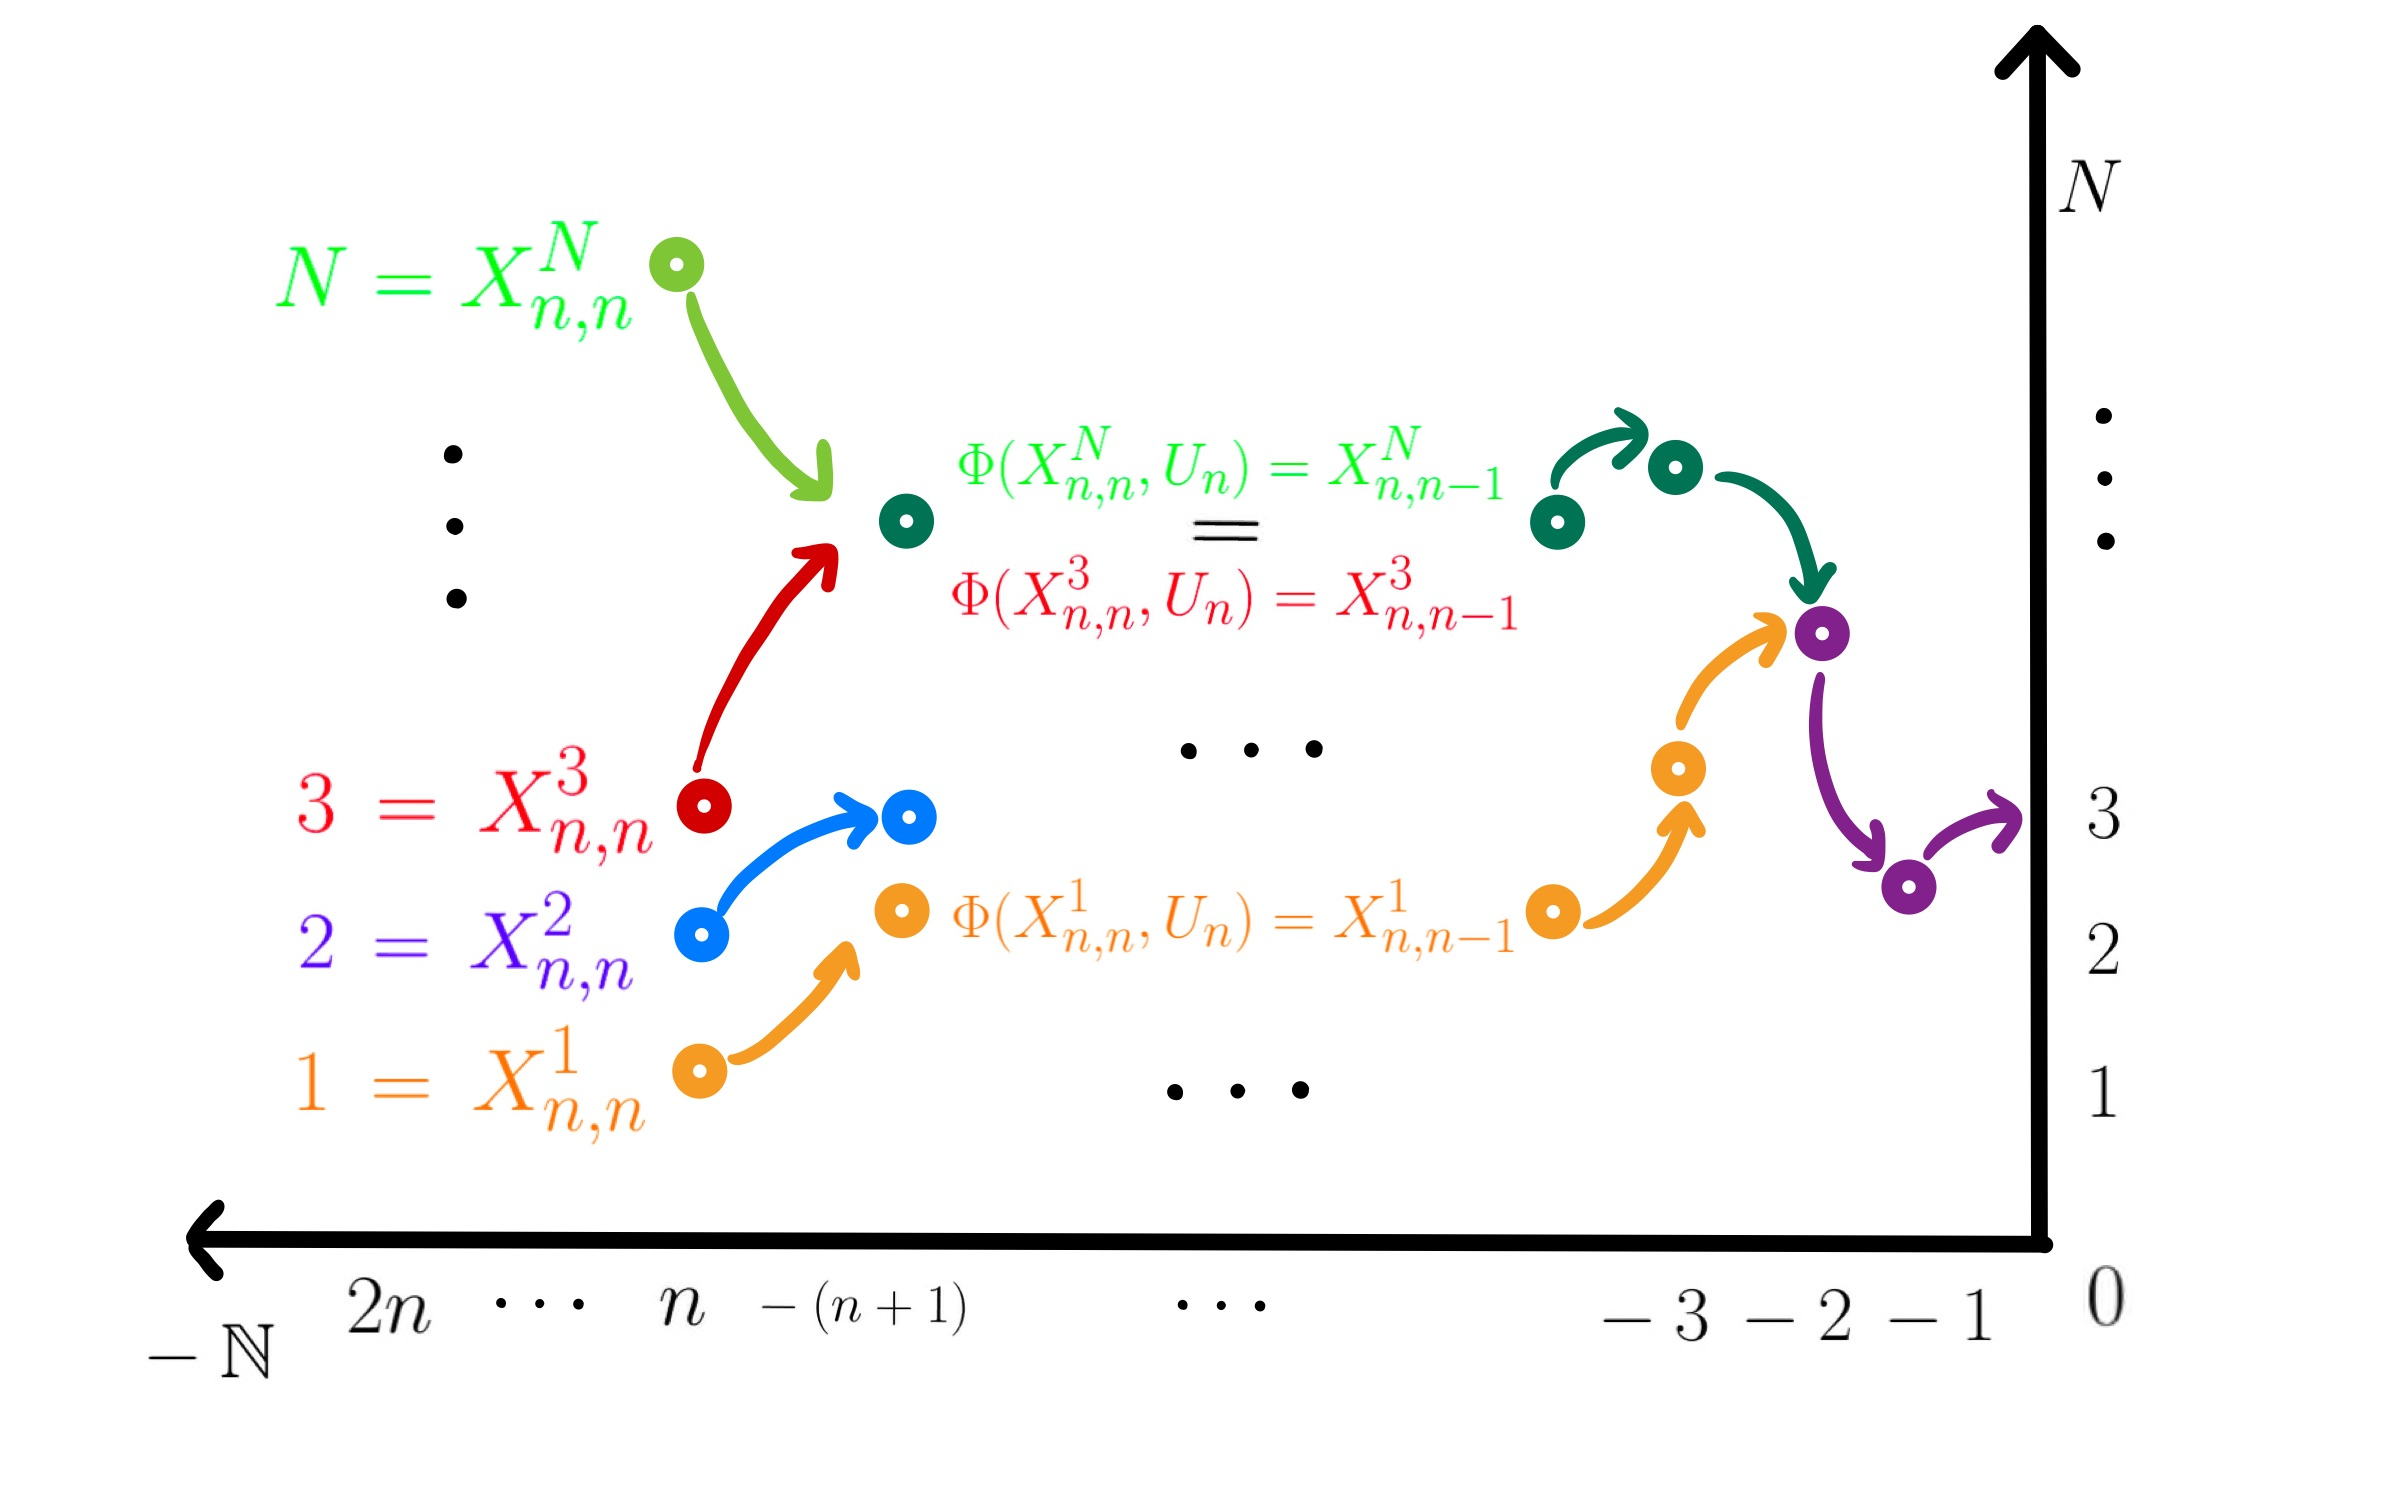
\includegraphics[scale=0.16]{img/clase_12_pag_9.jpg}
    \caption{Ejemplo de $(X^y_{n,m})_{m\geq n}$ que coalescen.}
    \label{fig:past}
\end{figure}

% \Huge
% $$ 3\, n\,-(n+1)\,2n\,-3\,-2\,-1\,-\N\,N$$
% $$ \color{orange} 1\,=\,X_{n,n}^1\,\Phi(X_{n,n}^1,U_n)=X^1_{n,n-1}$$
% $$ \color{blue} 2\,=\,X_{n,n}^2$$
% $$ \color{red} 3\,=\,X_{n,n}^3\,\Phi(X_{n,n}^3,U_n)=X^3_{n,n-1}$$
% $$ \color{green} N = X_{n,n}^N\,\Phi(X_{n,n}^N,U_n)=X^N_{n,n-1}$$


\iffalse  %%%%%%%%%%%%%%%%%
\begin{alignat*}{2}
    X^1_{n,m} & = \Phi^1_m(X^1_{n,m-1}) \\
    X^2_{n,m} & = \begin{cases}
        \Phi^2_m(X^2_{n,m-1}) & \mbox{ si }X^2_{n,m-1}\neq X^1_{n,m-1}\\
        \Phi^1_m(X^2_{n,m-1}) & \mbox{ si }X^2_{n,m-1}= X^1_{n,m-1}
    \end{cases} \\
    \vdots & \\
    X^y_{n,m} & = \begin{cases}
        \Phi^y_m(X^y_{n,m-1}) & \mbox{ si }X^y_{n,m-1}\notin\{ X^1_{n,m-1},\dots,X^{y-1}_{n,m-1}\}\\
        \Phi^{x_y}_m(X^y_{n,m-1}) & \mbox{ si }X^y_{n,m-1}\in\{X^1_{n,m-1},\dots,X^{y-1}_{n,m-1}\}
    \end{cases} \\
    \vdots & \\
    X^N_{n,m} & = \begin{cases}
        \Phi^N_m(X^N_{n,m-1}) & \mbox{ si }X^N_{n,m-1}\notin\{ X^1_{n,m-1},\dots,X^{N-1}_{n,m-1}\}\\
        \Phi^{x_N}_m(X^N_{n,m-1}) & \mbox{ si }X^N_{n,m-1}\in\{X^1_{n,m-1},\dots,X^{N-1}_{n,m-1}\}
    \end{cases}\, ,
\end{alignat*}
\fi  %%%%%%%%%%%%%%%%%%%%5
\vspace{.5cm}\\
\begin{theorem}
Si $\tau_o>-\infty$ c.s., se tiene 
$$X^y_{\tau_0,0}\sim\pi\espacio\forall y\in E \,.$$
\end{theorem}
\vspace{.5cm}\\
\begin{proof}  % min 38
\gris
$\forall k\in -\N$, $x,y\in E$
$$ \P(X^y_{\tau_0,0}=x,\tau_0>k) = \P(X^y_{k,0}=x,\tau_0>k) \,.$$
Luego $\P(X^y_{\tau_0,0}=x)=\displaystyle\lim_{k\to-\infty}\P(X^y_{k,0}=x)$. Por otro lado
\begin{alignat*}{2}
    |\P(X^y_{k,0}=x)-\pi_x| & = |\P(X_0=x|X_k=y)-\displaystyle\sum_z\pi_z\P(X_0=x|X_n=z)| \\
     & \leq \sum_{z}\pi_z|\P(X_0=x|X_k=y)-\P(X_0=x|X_k=z)|\,.
\end{alignat*}
En general, si $(V,W)$ es un coupling de dos leyes $\mu$ y $\nu$,
\begin{alignat*}{2}
\mu_y = \P(V=y) & = \P(V=y,W=y)+\P(V=y,W\neq y) \\
 & \leq \P(W=y)+\P(V\neq W) \\
 & = \nu_y + \P(V\neq W)\,. \\
 \therefore |\mu_y-\nu_y| & \leq \P(V\neq W) \\
 \therefore |\P(X^y_{k,0}=x)-\pi_x| & \leq \displaystyle\sum_z\pi_z\P(X^y_{k,0} \neq X^z_{k,0}) \\
 & \leq \P(\tau_0<k) \mbox{ }\substack{\longrightarrow \\ k\to-\infty}\mbox{ }0\, .
\end{alignat*}
Entonces,
$$ \P(X^y_{\tau,0}=x)=\mbox{ }\substack{\longrightarrow \\ k\to-\infty}\mbox{ }\P(X^y_{k,0}=x)=\pi_x \, .$$
\findem
\negro
\end{proof}
% \vspace{.5cm}\\
\subsubsection{Criterio Foster-Lyapunov para convergencia geométrica}
\begin{theorem}[de Harris]
Sea $(X_n)_{n\in\N}$ cadena de Markov en $E$ con matriz $P$ irreducible tal que
\begin{itemize}
    \item $\exists K\subseteq E$, $\exists\beta>0$, $m\in\mathcal{P}(E)$, $n_0\in\N$ tal que
    $$ (P^{n_0})_{xy}\geq\beta_{my}\espacio\forall x\in K,\,\forall y\in E \, .$$
    Esto es, una condición de tipo Doeblin (D) en $K$.
    \item $\exists V:E\longmapsto [1,\infty)$, $\rho\in(0,1)$, $c>0$ tal que
    $$ PV(x)\leq\rho V(x)+c\mathbf{1}_K(x) \espacio\forall x\in E \,.$$
    (Esta condición de ``tipo Lyapunov'' fuera de $K$ nos dice que $V$ tiende a decrecer en promedio.)
\end{itemize}
Entonces, $(X_n)_{n\in\N}$ es recurrente positiva, y $\exists\theta\in(0,1)$, $M>0$ tal que $\forall x\in E$
$$ \|P^n_{x_0}-\pi\|_1\leq M\theta^n \, ,$$
i.e., es uniformemente ergódica.
\end{theorem}
\vspace{.5cm}\\
Probaremos sólo un resultado intermedio:
\begin{lemma}
Sea $\tau_K=\inf\{n\geq1:X_n\in K\}$ tiempo de parada. Entonces $\forall x\notin K$,
$$ \E(\rho^{-\tau_K})<\infty \, .$$
\end{lemma}
\begin{remark}
Luego $\tau_K$ tiene un momento exponencial ($\rho^{-1}>1$), y $\forall n$
$$ \P_x(\tau_K>n)=\E_X(\mathbf{1}_{\tau_k>n})=\E_X(\mathbf{1}_{\rho^{-\tau_X}>\rho^{-n}})\leq\rho^n\E_X(\rho^{-\tau_k}) \, ,$$
i.e., $\tau_k$ tiene ``cola geométrica'' (y entonces toma valores grandes con baja probabilidad).
\end{remark}
\begin{proof}
\gris
Probaremos que $Y_n:=\rho^{-\min\{n,\tau_K\}}V(X_{\min\{n,\tau_K\}})$ es una sobre-martingala en la filtración $\mathcal{F}_n:=\sigma(X_0,\dots,X_n)$, esto es. $\E_x(Y_{n+1}|\mathcal{F}_n)\leq Y_n$. Como las esperanzas decrecen, $\E(Y_n)\leq E_x(Y_0)$, y dado que  $V(\cdot)\geq 1$, se obtendr\'a entonces que
$$ \E_x(\rho^{\min\{n,\tau_K\}})\leq\E_X(\rho^{\min\{n,\tau_K\}V(X_{\min\{n,\tau_K\}})})\leq V(x)<\infty \, . $$
Luego, tomando $n\to\infty$, por T.C.M. se concluye que  $\E_x(\rho^{-\tau_K})<\infty$. Estudiemos entonces  
\begin{alignat*}{2}
\E_x(Y_{n+1}|\mathcal{F}_n) & = \E_x(\rho^{-(n+1)}V(X_{n+1})\mathbf{1}_{\tau_K>n}|\mathcal{F}_n)+\E_x(\rho^{-\tau_K}V(X_{\tau_K})\mathbf{1}_{\tau_K\leq n}|\mathcal{F}_n) \, .
\end{alignat*}
El primer término queda
\begin{alignat*}{2}
\E_x(\rho^{-(n+1)}V(X_{n+1})\mathbf{1}_{\tau_K>n}|\mathcal{F}_n) & = \rho^{-(n+1)}\E(V(X_{n+1})|\mathcal{F}_n)\mathbf{1}_{\tau_K>n} \\
& = \rho^{-(n+1)}PV(X_n)\mathbf{1}_{\tau_K>n} \\
& \leq \rho^{-n}V(X_n)\mathbf{1}_{\tau_K>n}, 
\end{alignat*}
donde usamos la propiedad de Markov y que $X_n\notin K$ en $\{\tau_K>n\}$ (entonces  $c\mathbf{1}_{K}(x)=0$). Por otro lado en el segundo término podemos sacar la $\E(\cdot|\mathcal{F}_n)$ pues $\mathcal{F}(X_{\tau_K})\mathbf{1}_{\tau_K\leq n}$ es $\mathcal{F}_n$-medible. Luego
\begin{alignat*}{2}
\E_x(Y_{n+1}|\mathcal{F}_n) & \leq \rho^{-n}V(X_n)\mathbf{1}_{\tau_K>n}+\rho^{-\tau_K}V(X_{\tau_K})\mathbf{1}_{\tau_K\leq n} \\
& = \rho^{\min\{n,\tau_K\}}V(X_{\min\{n,\tau_K\}})=Y_n \, .
\end{alignat*}
\findem
\negro
\end{proof}
